\documentclass[dvipsnames,usenames,10pt]{beamer}

\usetheme{JuanLesPins}

\title{2APL: A Practical Programming Language and Platform for Multi-agent Systems}

\author[B. Borja Fiz, F. De Santis, M. Gabarda]{Beltran Borja Fiz, Fabrizio De Santis, Marcos Gabarda}
\institute[Universitat Polit\`ecnica de Catalunya]{
			Multi-agent Systems Course\\
			Master in Artificial Intelligence\\
			Universitat Polit\`ecnica de Catalunya\\
			\texttt{\\ \{beltran.borja.fiz, fabrizio.de.santis, marcos.gabarda\}@est.fib.upc.edu}}
\date{\today}

\setbeamercolor{exupcol}{fg=white,bg=NavyBlue}
\setbeamercolor{exlowcol}{fg=black,bg=NavyBlue!40}
\setbeamercolor{synupcol}{fg=white,bg=LimeGreen}
\setbeamercolor{synlowcol}{fg=black,bg=LimeGreen!40}
\setbeamercolor{semupcol}{fg=white,bg=Orange}
\setbeamercolor{semlowcol}{fg=black,bg=Orange!40}

\newcommand{\bsyntax}{\begin{beamerboxesrounded}[upper=synupcol,lower=synlowcol,shadow=true]{Formal Syntax}}
\newcommand{\esyntax}{\end{beamerboxesrounded}}

\newcommand{\bexample}{\begin{beamerboxesrounded}[upper=exupcol,lower=exlowcol,shadow=true]{Example}}
\newcommand{\eexample}{\end{beamerboxesrounded}}

\newcommand{\bopsem}{\begin{beamerboxesrounded}[upper=semupcol,lower=semlowcol,shadow=true]{Operational Semantics}}
\newcommand{\eopsem}{\end{beamerboxesrounded}}

\newcommand{\bformsem}{\begin{beamerboxesrounded}[upper=semupcol,lower=semlowcol,shadow=true]{Formal Semantics}}
\newcommand{\eformsem}{\end{beamerboxesrounded}}

\begin{document}

\frame{\titlepage}

\section*{Outline}

\frame{
	\frametitle{Outline}
	\tableofcontents
}
%%%%%%%%%%%%%%%%%%%%%%%%%%%%%%%%%%%%%%%%%%%%%%%%%%%%%%%%%%%%%%%%%%%%%%%%
\section{Introduction}	%%%% BORJA here
%%%%%%%%%%%%%%%%%%%%%%%%%%%%%%%%%%%%%%%%%%%%%%%%%%%%%%%%%%%%%%%%%%%%%%%%

\frame{
  \frametitle{Introduction}
 \begin{itemize}
  \item 2APL (double-a-p-l) is designed and developed at the Intelligent Systems Group at the University of Utrecht.
\item Designed in order to be "A Practical Agent Programming Language".
\item First version released in 2008. It is the successor of 3APL, and added multi-agent capabilities. It is built on the JADE platform.
\item It provides practical extensions with constructs that makes it easier to program in and debug

\begin{itemize}
  \item Testing, different execution modes, event and exception handling mechanism
  \item Supports the integration of declarative concepts (belief, goals) with imperative style programming (events, plans)
  \item Aims at improving the practical application of BDI agent programming language.
\end{itemize}
\end{itemize}  

}
%%%%%%%%%%%%%%%%%%%%%%%%%%%%%%%%%%%%%%%%%%%%%%%%%%%
\frame{
  \frametitle{2APL}
 \begin{itemize}
\item 2APL distinguishes itself from other agent-oriented programming languages by realising an effective integration of declarative and imperative style programming.

\item The declarative style programming supports the implementation of the mental state of agents allowing them to reason about their mental states and update them accordingly.

\item The imperative style programming supports the implementation of processes allowing programming constructs to implement both the flow of control as well as mechanisms such as procedure call, recursion, plan revision, and interface to existing imperative programming languages.

\end{itemize}
}

%%%%%%%%%%%%%%%%%%%%%%%%%%%%%%%%%%%%%%%%%%%%%%%%%%%
\frame[allowframebreaks]{
    \frametitle{2APL Features}
    
\begin{itemize}
    \item Programming Constructs:
     \begin{itemize}
        \item Multi-Agent System: Which and how many agents to create? Which
        environments? Which agent can access which environment?

         \item Individual Agent: Beliefs, Goals, Plans, Events, Messages

     \end{itemize}

     \item Programming Principles and Techniques:
     \begin{itemize}
        \item Abstraction: Procedures and Recursion in Plans
        \item  Error Handling: Plan Failure and their revision by Internal Events,
        \item Execution of Critical Region of Plans
        \item  Legacy Systems: Environment and External Actions
        \item  Encapsulation: Including 2APL ¯les in other 2APL ¯les
        \item  Autonomy: Adjustable Deliberation Process
    \end{itemize}
\end{itemize}

\break

\begin{itemize}
    \item Integrated Development Environment
     \begin{itemize}
        \item 2APL platform is Built on JADE and uses related tools
        \item Editor with High-Lighting Syntax
        \item Monitoring mental attitudes of individual agents, their reasoning and
communications
        \item Executing in one step or continuous mode
        \item Visual Programming of the Deliberation Process

    \end{itemize}
\end{itemize}

}

%\frame{
%	\frametitle{Introduction}
%	
%	2APL is designed and developed at the Intelligent Systems Group at the University of Utrecht.

%	\begin{itemize}
%		\item It is a BDI-based agent-oriented programming language that integrates
%		\begin{itemize}
%			\item \emph{declarative} programming constructs such as belief and goals
%			\item \emph{imperative} style programming constructs such as events and plans
%		\end{itemize}
%	\end{itemize}
%}

%\frame{
	%\frametitle{History}
%}

%\frame[allowframebreaks]{
  %\frametitle{Prolog Introduction}

  %% a short introduction to Prolog
  %Prolog is a general purpose logic programming language.

  %% horn clauses
  %Based on Horn Clauses
  %\begin{itemize}
    %\item $H \leftarrow B_{1} \wedge \ldots \wedge B_{n}$
    %\item $H \leftarrow true$
  %\end{itemize}

  %\break

  %\begin{itemize}
    %% data types
    %\item {\bf Data Types}
    %\begin{itemize}
      %\item Atoms, general-purpose name with no inherent meaning. Atoms include x, red, 'Ball', and 'some atom'.
      %\item Numbers, integer or float.
      %\item Variables, denoted by a string beginning with an upper-case letter or underscore.
      %\item Compound Term, composed of an atom called a "functor" and a number of "arguments".
    %\end{itemize}
    %% rules and facts
    %\item {\bf Rules and Facts}
    %\begin{itemize}
      %\item Rule: \texttt{Head :- Body.}
      %\item Fact: \texttt{father(sam).}
    %\end{itemize}
  %\end{itemize}

  %\break

  %% evaluation
  %\begin{itemize}
    %\item {\bf Evaluation}
    %\begin{itemize}
      %\item Execution of a Prolog program is initiated by the user's posting of a single goal, called the query
      %\item The Prolog engine tries to find a resolution refutation of the negated query
      %\item The resolution method used by Prolog is called {\bf SLD resolution}
    %\end{itemize}
  %\end{itemize}
%}

%%%%%%%%%%%%%%%%%%%%%%%%%%%%%%%%%%%%%%%%%%%%%%%%%%%%%%%%%%%%%%%%%%%%%%%%
\section{2APL Language} % Fabrizio
%%%%%%%%%%%%%%%%%%%%%%%%%%%%%%%%%%%%%%%%%%%%%%%%%%%%%%%%%%%%%%%%%%%%%%%%

\subsection{Syntax and operational semantics}

\frame{
	\frametitle{2APL Language}
	
	There are 2 distinguished set of programming constructs for defining:
	
	\vskip 2.0ex
	
	\begin{enumerate}
		\item Multi-agent system 
		\item Individual agents
	\end{enumerate}	
}

\subsubsection{Multi-agent system specification}

\begin{frame}[allowframebreaks,fragile]
	\frametitle{Multi-agent system specification}

	A multi-agent system is specified by a set of couples:

	\vskip 2.0ex
	
	\begin{enumerate}
		\item Individual agent
		\item Environments they have access to
%		\begin{itemize}
%			\item Java class with an internal a state
%			\item A set of actions (methods) to change the state
%			\item Can function as interface (e.g. real world, other software)
%		\end{itemize}		
	\end{enumerate}

	\break	

\bsyntax 
\begin{verbatim}
<MAS_Prog>     := ( <agentname> ``:'' <filename> [<int>]
                   [<environments>] )+
<agentname>    := <ident>
<filename>     := <ident>``.2apl''
<environments> := ``@''<ident> (``,'' <ident>)*
\end{verbatim}
\esyntax

	\vskip 1.0ex
	
\bexample
\begin{verbatim}
harry : harry.2apl @blockworld
sally : sally.2apl @blockworld
\end{verbatim}
\eexample
\end{frame}

\subsubsection{Individual agent specification}

\frame[allowframebreaks]{
	\frametitle{Individual agent specification}
	
	2APL agents are implemented in terms of:

	\vskip 2.0ex

	\begin{itemize}
		\item beliefs	
		\item goals	
		\item actions
		\item plans
		\item events
		\item 3 kind of different practical reasoning rules for
			\begin{itemize}
				\item Generating plans for achieving goals
				\item Processing events and messages
				\item Handling and repairing failed plans
			\end{itemize}			
	\end{itemize}	
	
	\vskip 2.0ex

%	The beliefs, goals, plans and reasoning rules form the \emph{mental states} of the 2APL agent.

	%Agent can observe an environment either:
	%\begin{itemize}
		%\item actively by means of a sense action
		%\item passively by means of events generated by the environment
	%\end{itemize}
	
	\break
	
	\bsyntax
	\begin{verbatim}
	<Agent_Prog> := ( ``Include:'' <ident>
	                | ``BeliefUpdates:'' <BelUpSpec>
	                | ``Beliefs:'' <belief> 
	                | ``Goals:'' <goals> 
	                | ``Plans:'' <plans>
	                | ``PG-rules:'' <pgrules>
	                | ``PC-rules:'' <pcrules>
	                | ``PR-rules:'' <prrules>
	                )*
	\end{verbatim}
	\esyntax
}

\frame[allowframebreaks]{
	\frametitle{Basic elements of the language}

	\begin{itemize}
		\item \texttt{<atom>}: Prolog like atomic formula starting with a lowercase letter
		\begin{itemize}
			\item Prolog formulas
		\end{itemize}
		\vskip 2.0ex
		\item \texttt{<Atom>}: Prolog like atomic formula starting with a capital letter
		\begin{itemize}
			\item Function names
		\end{itemize}
		
		\break
		
		\item \texttt{<ground\_atom>}: grounded atomic formula
		\begin{itemize}
			\item Prolog formulas that does not contain any variables
		\end{itemize}
		\vskip 2.0ex
		\item \texttt{<Var>}: string with a capital letter
		\begin{itemize}
			\item Variables
		\end{itemize}
		\vskip 2.0ex
		\item \texttt{<ident>}: string with a lowercase letter
	\end{itemize}
}

\frame{
	\frametitle{Beliefs and goals}

	A 2APL agent has \emph{beliefs} and \emph{goals} that may change during the execution

	\vskip 2.0ex
	
	\begin{itemize}
		\item Beliefs are containted into a \emph{belief base} and they are related to:
			\begin{itemize}
				\item The environment
				\item Other agents
			\end{itemize}
		\item Goals are contained into a \emph{goal base}
	\end{itemize}
	
	\vskip 2.0ex

	Rationality principle: if an agent believes a certain fact, then it can not purse that fact as a goal	
%	\begin{itemize}
%		\item If an agent modifies its belief base, then its goal base may require a modification
%	\end{itemize}
		
}

\begin{frame}[fragile,allowframebreaks]
	\frametitle{Belief base}

	\bsyntax
	\begin{verbatim}
	``Beliefs:'' <belief>
	
	<belief>   := ( <ground_atom> ``.''
	              | <atom> ``:-'' <literals> ``.'' 
	              )+
	<literals> := <literal> (``,'' <literal>)*
	<literal>  := ( <atom> 
	              | ``not'' <atom>
	              )
	\end{verbatim}
	\esyntax

	\vskip 1.0ex
	
	\begin{itemize}
		\item Actually, a belief base is a Prolog program
		\begin{itemize}
			\item Each belief is a Prolog fact or rule
			\item All facts are assumed to be grounded
		\end{itemize}
	\end{itemize}

	\break
	
	\bexample
	\begin{verbatim}
	Beliefs:
	       bomb(3,4).
	       clean(blockWorld) :- not bomb(X,Y), not carry(bomb).
	\end{verbatim}
	\eexample
\end{frame}

\begin{frame}[fragile]
	\frametitle{Goal base}
	
	\bsyntax 
	\begin{verbatim}
	``Goals:'' <goals>
	
	<goals> := <goal> ( ``,'' <goal> )*
	<goal>  := <ground_atom> ( ``and'' <ground_atom> )*
	\end{verbatim}
	\esyntax
	
	\vskip 1.0ex

	Each goal expression is a conjunction of ground atoms. 
	
	\vskip 1.0ex
	
	\bexample
	\begin{verbatim}
	Goals:
	     clean(blockWorld)
	\end{verbatim}
	\eexample
	
	\begin{itemize}
		\item Having ``\texttt{a and b}'' is different than having ``\texttt{a, b}''
		\item Goal base is a list such that the goals are ordered
	\end{itemize}
\end{frame}

\begin{frame}[fragile,allowframebreaks]
	\frametitle{Basic actions}
	
	A 2APL agent needs to act in order to achieve its goals.

	\vskip 2.0ex
	
	There are 6 types of basic actions:
	
	\begin{enumerate}
		\item Belief base update action
		\item Communication action
		\item External action
		\item Abstract action
		\item Test actions
		\item Goal dynamic actions
	\end{enumerate}
	
	\break
	
	\bsyntax
	\begin{verbatim}
	<baction> = ( ``skip'' | <beliefupdate>
	            | <sendaction> | <externalaction> 
	            | <abstractaction> | <test>
	            | <adoptgoal> | <dropgoal>
	            )
	\end{verbatim}
	\esyntax

	%\vskip 2.0ex

	%The execution of a \texttt{skip} action always succeeds resulting in its removal from the plan base
\end{frame}

\begin{frame}[fragile,allowframebreaks]
	\frametitle{Belief update action}
	
	\bsyntax
	\footnotesize
	\begin{verbatim}
	``BeliefUpdates:'' <BelUpSpec>
	
	<BelUpSpec>    := (
	                  ``{'' <belquery> ``}''
	                      <beliefupdate>
	                  ``{'' <literals> ``}''
	                  )+
	<belquery>     := ( ``true'' 
	                  | <belquery> ``and'' <belquery>
	                  | <belquery> ``or'' <belquery>
	                  | ``('' <belquery> ``)''
	                  | <literal>
	                  )
	<beliefupdate> := <Atom>
	\end{verbatim}
	\esyntax
	
	\vskip 2.0ex
	
	Updates the belief base using precondition-delete-add formalism.

	\break

	\bexample
	\begin{verbatim}
	BeliefUpdates:
	  { bomb(X,Y) }       RemoveBomb(X,Y) { not bomb(X,Y) }
	  { true }            AddBomb(X,Y)    { bomb(X,Y) }
	  { carry(bomb) }     Drop()          { not carry(bomb) }
	  { not carry(bomb) } PickUp()        { carry(bomb) }
	\end{verbatim}
	\eexample

	\vskip 2.0ex
	
	\begin{itemize}
		\item The specification of belief update actions does not change during agent execution
		\item After the execution of the action, the post-condition is entailed by the belief base
	\end{itemize}
\end{frame}

\begin{frame}[fragile,allowframebreaks]
	\frametitle{Communication action}
	
	A communication action passes a message to another agent.
	
	\vskip 1.0ex
	
	% formal syntax
	\bsyntax
	\small
	\begin{verbatim}
	<sendaction> := ``send('' <iv> ``,'' <iv> ``,''
	                        [ <iv> ``,'' <iv> ``,'' ]  <atom> ``)''  
	<iv>         := <ident> | <Var>
	\end{verbatim}
	\esyntax

	\vskip 1.0ex

	% operational semantics
%	\bopsem
	\begin{verbatim}
	send(Receiver, Performative, Language, Ontology, Content)
	or
	send(Receiver, Performative, Content)
	\end{verbatim}
%	\eopsem

	\vskip 1.0ex

	% example
	\bexample
	\begin{verbatim}
	send(harry, inform, La, On, bombAt(X1,Y1))
	\end{verbatim}
	\eexample
\end{frame}

\begin{frame}[fragile]
	\frametitle{External action}
	
	An external action is \emph{supposed} to change the state of an external environment
	
	\vskip 2.0ex
	
	\begin{itemize}
		\item Effects of actions are assumed to be determined by the environment
		\item A sense action needs to be performed to determine an effect
	\end{itemize}	
	
	\bsyntax
	\small
	\begin{verbatim}
	<externalaction> := ``@'' <ident> ``('' <atom> ``,'' <Var> ``)''
	\end{verbatim}
	\esyntax

	\vskip 1.0ex

%	\bopsem
	\begin{verbatim}
	@Env(ActionName, Return, Time-out)
	\end{verbatim}
%	\eopsem

	\vskip 1.0ex

	\bexample
	\begin{verbatim}
	@blockworld(east(), L)
	\end{verbatim}
	\eexample
\end{frame}

\begin{frame}[fragile]
	\frametitle{Abstract action}
	
	\bsyntax
	\begin{verbatim}
	<abstractlaction> := <atom>
	\end{verbatim}
	\esyntax

	\vskip 2.0ex

	\begin{itemize}
		\item It is similar to a procedure call
		\item It substitutes the current execution of a plan with the instantiation of another plan
	\end{itemize}
\end{frame}

\begin{frame}[fragile,allowframebreaks]
	\frametitle{Test actions}
	
	Test actions are query expressions used to check if an agent can derive certain beliefs and goals from its bases.

	\vskip 2.0ex
	
	\bsyntax
	\small
	\begin{verbatim}
	<test>      := ( ``B('' <belquery> ``)'' 
	               | ``G('' <goalquery> ``)''
	               | <test> ``&'' <test>
	               )
	<goalquery> := ( ``true'' 
	               | <goalquery> ``and'' <goalquery>
	               | <goalquery> ``or'' <goalquery>
	               | ``('' <goalquery> ``)''
	               | <atom>
	               )
	\end{verbatim}
	\esyntax
	
	\break

	\bexample
	\begin{verbatim}
	p(a)                       // belief
	...
	q(b)                       // goal
	...
	B(p(X)) & G(q(X))          // fails	
	B(p(X)) & G(q(Y) or r(X))  // success by {X/a, Y/b}
	\end{verbatim}
	\eexample
\end{frame}

\begin{frame}[fragile,allowframebreaks]
	\frametitle{Goal dynamics actions}
	
	They are used to adopt and drop goals to and from an agent's goal base.

	\vskip 2.0ex

	\bsyntax
	\footnotesize
	\begin{verbatim}
	<adoptgoal> := ( ``adopta('' <goalvar> ``)''
	               | ``adoptz('' <goalvar> ``)''
	               )
	<dropgoal>  := ( ``dropgoal('' <goalvar> ``)''
	               | ``dropsubgoals('' <goalvar> ``)''
	               | ``dropsupergoals('' <goalvar> ``)''
	               )
	<goalvar>   := ( <atom> | ``not'' <atom> )
	\end{verbatim}
	\esyntax

	\vskip 2.0ex
	
	%It is programmer task to ensure that the variables are instantiated before the actions are executed.

	\break

	\bexample
	\footnotesize
	\begin{verbatim}
	// Goal base
	a(1)
	a(1) and b(1)
	a(1) and b(1) and c(1)

	...

	dropgoal(a(1) and b(1))       // drops a(1) and b(1)
	dropsubgoal(a(1) and b(1))    // drops a(1), a(1) and b(1)
	dropsupergoal(a(1) and b(1))  // drops a(1) and b(1), a(1) and b(1) and c(1)
	\end{verbatim}
	\eexample
\end{frame}

\begin{frame}[fragile,allowframebreaks]
	\frametitle{Plans}
	
	In order to reach its goals, a 2APL agent adopts \emph{plans}.

	\vskip 2.0ex
	
	A plan consists of basic actions that can be composed by using different operators:
	\begin{itemize}
		\item sequence operator
		\item conditional choice operators
		\item conditional iteration operator
		\item atomic operator for plans that must be executed atomically
	\end{itemize}	

	\vskip 2.0ex

	An agent can have different plans at the same time.

	\break	

	\bsyntax
	\small
	\begin{verbatim}
	<plan>         := ( <baction> | <sequenceplan>
	                  | <ifplan> | <whileplan>
	                  | <atomicplan>
	                  )
	<sequenceplan> := <plan> ``;'' <plan>
	<ifplan>       := ``if'' <test> ``then'' <scopeplan>
	                 [``else'' <scopeplan>]
	<scopeplan>    := ``{'' <plan ``}''
	<whileplan>    := ``while'' <text> ``do'' <scopeplan>
	<atomicplan>   := ``['' <plan> ``]''
	\end{verbatim}
	\esyntax
\end{frame}

\begin{frame}[fragile]
	\frametitle{Plan base}

	The plans of a 2APL agent are implemented by its plan base.
	
	\vskip 2.0ex

	\bsyntax
	\begin{verbatim}
	Plans: <plans>

	<plans> := <plan> ( ``,'' <plan> )*
	\end{verbatim}
	\esyntax

	\vskip 2.0ex

	Initial plan base:

	\vskip 2.0ex

	\bexample
	\begin{verbatim}
	Plans:

	B(start(X,Y)) ; @blockworld(enter(X, Y, blue), L)
	\end{verbatim}	
	\eexample
\end{frame}

\begin{frame}
	\frametitle{Reasoning rules}

	3 \emph{practical} reasoning rules are used for generating plans.	

	\vskip 2.0ex

	\begin{enumerate}
		\item Planning goal rules (PG rules)
		\item Procedural rules    (PC rules)
		\item Plan repair rules   (PR rules)
	\end{enumerate}
\end{frame}

\begin{frame}[fragile,allowframebreaks]
	\frametitle{Planning goal rules}

	They are used to generate plans starting from certain beliefs and goals.

	\vskip 2.0ex

	\bsyntax
	\begin{verbatim}
	``PG-rules:'' <pgrules>
	
	<pgrules> := <pgrule>+
	<pgrule>  := [<goalquery>] ``<-'' <belquery> ``|'' <plan>
	\end{verbatim}
	\esyntax

	\break

	\bexample 
	\begin{verbatim}
	PG-rules:
	clean(blockWorld) <- bomb(X, Y) | { 
	goto(X, Y);                  // abstract action
	@blockworld(pickup(), L1);   // external action
	PickUp();                    // belief update action
	RemoveBomb(X, Y);

	goto(0, 0);
	@blockworld(drop(), L2);
	Drop();
	}
	\end{verbatim}
	\eexample
\end{frame}

\begin{frame}[fragile,allowframebreaks]
	\frametitle{Procedural rules}

	They are used to generate plans as a response to:

	\begin{enumerate}
		\item the execution of abstract actions
		\item the reception of
		\begin{itemize}
			\item messages from other agents
			\item events generated by the external environment or internally
		\end{itemize}
	\end{enumerate}

	\break
	
	\vskip 2.0ex

	\bsyntax
	\begin{verbatim}
	``PC-rules:'' <pcrules>
	
	<pcrules> = <pcrule>+
	<pcrule> = <atom> ``<-'' <belquery> ``|'' <plan>
	\end{verbatim}
	\esyntax

	\vskip 2.0ex

	A PC rule is applied iif the belief condition is entailed by the belief base.

	\break

	\bexample
	\footnotesize
	\begin{verbatim}
	PC-rules:
	goto(X, Y) <- true | {
	  @blockworld(sensePosition(), POS);
	  B(POS = [A,B]);
	  if B(A > X) then {
	     @blockworld( west(), L);
	     goto(X, Y);
	  } else if B(A < X) then {
	     @blockworld( east(), L);
	     goto(X, Y);
	  } else if B(B > Y) then {
	     @blockworld( north(), L);
	     goto(X, Y);
	  } else if B(B < Y) then {
	    @blockworld(south(), L);
	    goto(X, Y);
	  }
	}
	\end{verbatim}
	\eexample
	
	\break

	\bexample
	\begin{verbatim}
	message(sally, inform, La, On, bombAt(X, Y)) <- true | {
	  if B(not bomb(A, B)) then { 
	    AddBomb(X, Y);
	    adoptz(clean(blockWorld));
	  } else { 
	    AddBomb(X, Y);
	  }
	}
	\end{verbatim}
	\eexample
\end{frame}

\begin{frame}[fragile,allowframebreaks]
	\frametitle{Plan repair rules}

	They are used to replace a plan whose execution has failed.

	\vskip 2.0ex

	\bsyntax
	\footnotesize
	\begin{verbatim}
	``PR-rules:'' <prrules>

	<prrules>      := <prrule>+
	<pcrule>       := <planvar> ``<-'' <belquery> ``|'' <planvar>
	<planvar>      := ( <plan>
	                  | <Var>
	                  | ``if'' <test> ``then'' <scopeplanvar>
	                   [``else'' <scopeplanvar>]
	                  | ``while'' <test> ``do'' <scopeplanvar> 
	                  | <planvar> ``;'' <planvar>
	                  )
	<scopeplanvar> := ``{'' <planvar> ``}''
	\end{verbatim}
	\esyntax

	\break

	It can be applied iif:
	\begin{enumerate}
		\item the execution of a plan fails
		\item there is rule matching the failed action
		\item the belief query expression is derivable from the agent's belief base
	\end{enumerate}

	\vskip 2.0ex
	
	\bexample
	\footnotesize
	\begin{verbatim}
	PR-rules: 
	@blockworld(pickup(), L) ; REST <− true | { 
	    @blockworld(sensePosition(), POS);
	    B(POS = [X, Y]);     // test action	
	    RemoveBomb(X, Y);    // belief update action
	}
	\end{verbatim}
	\eexample

	\vskip 2.0ex
	
	\texttt{REST}: the rest of the original plan is dropped.

	\break

	When the execution of a plan fails?

	\vskip 2.0ex

	It depends on the type of the action
	\begin{itemize}
		\item Belief update action
			\begin{itemize}
				\item  It is not specified or the pre-condition is not entailed by the belief base
			\end{itemize}
		\item Abstract action
			\begin{itemize}
				\item There is no applicable procedural rule 
			\end{itemize}
		\item External action
			\begin{itemize}
				\item The environment throws an \texttt{ExternalActionFailedException}
				\item The agent has no access to the environment
				\item The actions is not defined in the environment
			\end{itemize}

		\break

		\item Test action 
			\begin{itemize}
				\item The test expression is no derivable from the belief or goal bases
			\end{itemize}
		\item Goal adopt action
			\begin{itemize}
				\item The goal is already entailed by the belief base
				\item The goal to be adopted is not ground
			\end{itemize}
		\item Atomic plan
			\begin{itemize}
				\item If one of its actions fails
			\end{itemize}
	\end{itemize}

	\vskip 2.0ex

	The execution of all other actions will be always successful.
	
\end{frame}

\subsubsection{Programming the environment}

\begin{frame}[fragile,allowframebreaks]
	\frametitle{Programming external environment}

	2APL environment can be any Java class implementing the \emph{environment interface}

	\vskip 2.0ex

	It contains the following methods:

	\begin{itemize}
		\item \texttt{addAgent(String name)}
		\item \texttt{removeAgent(String name)}
	\end{itemize}

	\vskip 2.0ex

	Any external action \texttt{@env($a_1, \ldots, a_n$, R)} is translated into a call to a method $m$ with arguments $a_1, \ldots, a_n$ in environment $env$

	\break

	\bexample
	\small
	\begin{verbatim}
	public Term move(String agent, String direction)
	   throws ExternalActionFailedException {
   	   
	   if (direction.equals("north") { moveNorth(); }
   	   else if (direction.equals("east") {moveEast(); }
   	   else if (direction.equals("south") {moveSouth(); }
   	   else if (direction.equals("west") {moveWest(); }
   	   else throw
	        new ExternalActionFailedException("Unknown direction");

   	   return getPositionTerm();
	}
	\end{verbatim}
	\eexample
\end{frame}

\frame[allowframebreaks]{
	\frametitle{Events and exceptions}
	
	\begin{itemize}
	\item \emph{Events} are used to pass information from environments to agents

	\vskip 2.0ex

	The programmer can decide when and which information from the environment pass to agents using:
	
	\vskip 2.0ex

	\texttt{notifyEvent(AF event, String ... agents)}

	\vskip 2.0ex

	\item The \emph{exception} are used to inform that an action has failed.
	\end{itemize}
}

\begin{frame}[fragile]
	\frametitle{Including 2APL files}

	Different agents may \emph{share} certain initial beliefs, goals, plans, belief updates, and practical reasoning rules.

	\vskip 2.0ex

	\bexample
	\begin{verbatim}
	Include: person.2apl    // implements goto(X,Y)
	\end{verbatim}
	\eexample
\end{frame}

%%%%%%%%%%%%%%%%%%%%%%%%%%%%%%%%%%%%%%%%%%%%%%%%%%%%%%%%%%%%%%%%%%%%%%%%
\subsection{Formal Semantics}
%%%%%%%%%%%%%%%%%%%%%%%%%%%%%%%%%%%%%%%%%%%%%%%%%%%%%%%%%%%%%%%%%%%%%%%%

\frame{
  \frametitle{Formal Semantics}

  % the objective of the formal semantics is to valitade the program across the specifications
  With formal semantics, it is possible to verify whether agent programs
  satisfy their (formal) specifications.

  % definition of the theoretical model as a transition system.
  \begin{itemize}
    \item The semantics of 2APL in terms of a {\bf transition system}.
    \item A {\bf transition system} is a set of transition rules for deriving
          {\bf transitions}.
    \item A {\bf transition} is a transformation of one {\bf configuration} into
          another and it corresponds to a single computation/execution step.
  \end{itemize}

  Elements to formal define:
  \begin{itemize}
    \item Configuration of individual 2APL agent.
    \item Configuration of multi-agent systems.
    \item Transitions.
  \end{itemize}

}

\frame[allowframebreaks]{
  \frametitle{Individual 2APL agent}

  An individual 2APL agent if defined as follow:

  % formal definition of an agent
  $$ A_{\iota} = \langle \iota, \sigma, \gamma, \Pi, \theta, \xi \rangle $$

  where $\iota$ is an agent id, $\sigma$ is a set of beliefs,
  $\gamma$ is a list of goals, $\Pi$ is a set of plans, $\theta$ is ground
  substitution and $\xi$ is the event base.

  \vskip 1.0ex

  $\xi = \langle E, I, M \rangle$ is the agent's event base, where:
  \begin{itemize}
    \item {\bf E} is a set of external events.
    \item {\bf I} is a set of plan identifiers denoting failed plans.
    \item {\bf M} is a set of messages sent to agent.
  \end{itemize}

  \break

  Each plan entry is a tuple $(\pi, r, p)$, where $\pi$ is the executing plan,
  $r$ is the instantiation of the PG-rule through which $\pi$ is generated, and
  $p$ is the plan identifier.

  \vskip 1.0ex

  The belief base and each goal in the goal base are only positive atoms.

}

\frame{
  \frametitle{Multi-agent Systems}

  The configuration of a 2APL multi-agents system is defined as:

  % formal definition of a multi-agent system
  $$ \langle A_{1}, \ldots, A_{n}, \chi \rangle $$

  where $\chi$ is a set of external shared environments.

}


\frame{
  \frametitle{Transitions}
  
  Transitions rules for basic actions:
  \begin{itemize}
    \item Skip action.
    \item Belief update actions.
    \item Test actions.
    \item Goal dynamics actions.
    \item Abstract actions.
    \item Communication actions.
    \item External actions.
  \end{itemize}

}

\frame{
  \frametitle{Skip actions}

  The execution of skip action has no effect on an agent's configuration. The
  execution of this action always succeeds resulting in its removal from the
  plan base.

  % formal application of the action
  $$ {{\gamma \vDash_{g} G(r)}\over{\langle \iota, \sigma, \gamma, \{(\texttt{skip}, r, id)\}, \theta, \xi \rangle  \rightarrow \langle \iota, \sigma, \gamma, \{\}, \theta, \xi \rangle}}$$

}

\frame{
  \frametitle{Belief update actions}

  A {\bf belief update action}:
  \begin{itemize}
    \item Is specified in terms of a pre- and a post-condition.
    \item Modifies the belief base when it is executed.
  \end{itemize}

  % formal application of the action
  $$ {{T(\alpha \theta, \sigma) = \sigma' \& \gamma \vDash_{g} G(r)} \over {\langle \iota, \sigma, \gamma, \{(\alpha, r, id)\}, \theta, \xi \rangle  \rightarrow \langle \iota, \sigma', \gamma', \{\}, \theta, \xi \rangle}} $$

  A belief update action can be executed if its pre-condition is
  entailed by the belief base.

  After the execution of the action, its
  post-condition should be entailed by the belief base.

}


\frame{
  \frametitle{Test actions}
  
  A test action checks if the belief and goal queries within a test expression
  are entailed by the agent's belief and goal bases.

%   Moreover, as some of the variables that
%   occur in the belief and goal queries may already be bound by the substitution θ , we apply the
%   substitution to the test expression before testing it against the belief and goal bases. After
%   applying θ , the test expression can still contain unbound variables (to bind next occurrences
%   of the variable in the plan in which it occurs). Therefore, the test action results in a substitution
%   τ which is added to θ .

  % formal application of the action
  $$ {{( \sigma, \gamma) \vDash_{t} \varphi \theta \tau \& \gamma \vDash_{g} G(r)}\over{\langle \iota, \sigma, \gamma, \{(\varphi, r, id)\}, \theta, \xi \rangle  \rightarrow \langle \iota, \sigma, \gamma, \{\}, \theta \cup \tau, \xi \rangle}} $$

  A test action can fail if one or more of its involved query expressions are not entailed by
  the belief or goal bases.

}

\frame[allowframebreaks]{
  \frametitle{Goal dynamics action}

  Goals can be adopted and added to the agent's goal base by means of basic
  actions {\tt adopta($\phi$)} and {\tt adoptz($\phi$)}.

  The first action adds the goal $\phi$ to the beginning of the goal base and the
  second action adds the  goal $\phi$ to the end of the goal base.
  % formal application of the action
  $$ {{{\sigma \nvDash \phi \theta} \& {\texttt{ground}(\phi \theta)} \& {\gamma \vDash_{g} G(r)}}\over{\langle \iota, \sigma, \gamma, \{(\texttt{adoptX}(\phi), r, id)\}, \theta, \xi \rangle  \rightarrow \langle \iota, \sigma, \gamma', \{\}, \theta, \xi \rangle}} $$

  \break

  Goals can be dropped and removed from the goal base by means of {\tt dropgoal($\phi$)},
  {\tt dropsubgoals($\phi$)}, and {\tt dropsupergoals($\phi$)} actions.

  The first action removes from the goal base the goal $\phi$, the second removes
  all goals that are subgoals of $\phi$, and the third action removes all goals that
  have $\phi$ as a subgoal.
  % formal application of the action
  $$ {{\gamma \vDash_{g} G(r)} \over {\langle \iota, \sigma, \gamma, \{(\texttt{dropX}(\phi), r, id)\}, \theta, \xi \rangle  \rightarrow \langle \iota, \sigma, \gamma', \{\}, \theta, \xi \rangle}} $$

}

\frame{
  \frametitle{Abstract actions}

  % Abstract actions can be used for different purposes. It can be used as a mechanism to reuse plans that occur
  % in many other plans, or they can be used to implement recursion.

  Abstract actions are representations of plans. The execution of an abstract
  action replaces the action with the plan it represents.

  % formal application of the action
  $$ {{Unify(\alpha\theta, \phi = \tau_{1} \& \sigma \vDash \beta\tau_{1}\tau_{2} \& \gamma \vDash_{g} G(r) } \over {\langle \iota, \sigma, \gamma, \{(\alpha, r, id)\}, \theta, \xi \rangle  \rightarrow \langle \iota, \sigma, \gamma', \{(\pi\tau_{1}\tau_{2}, r, id)\}, \theta, \xi \rangle}} $$

}

\frame{
  \frametitle{Communication actions}

  Agents can communicate with each other by sending messages to each other.
  An agent can send a message to another agent by means of the
  \texttt{send}(j, p, l, o, $\phi$) action. The execution of the send action
  broadcasts a message which will be added to the event base of the receiving
  agent.

  \vskip 1.0ex

  The execution of the send action broadcasts a message which will be added to
  the event base of the receiving agent. The broadcasted message will include
  the name of the sending agent.


  % formal application of the action
  $$ $$

}

\frame{
  \frametitle{External actions}

  The execution of an external action by an individual agent affects the
  external environments that may be shared by other agents.

  % formal application of the action
  $$ $$

}

\frame{
  \frametitle{Transitions}

  Transitions rules for plans:
  \begin{itemize}
    \item Sequence plan.
    \item Conditional plan.
    \item While plan.
    \item Atomic plan.
    \item Multiple concurrent plans.
  \end{itemize}

}

\frame{
  \frametitle{Sequence Plan}

  The execution of a sequence plan $\alpha; \pi$ consists of the execution of
  the basic action $\alpha$ followed by the execution of plan $\pi$.

  % formal application of the action
  $${ {\langle \iota, \sigma, \gamma, \{(\alpha, r, id)\}, \theta, \xi \rangle  \rightarrow \langle \iota', \sigma', \gamma, \{\}, \theta', \xi' \rangle} \over {\langle \iota, \sigma, \gamma, \{(\alpha:\pi, r, id)\}, \theta, \xi \rangle  \rightarrow \langle \iota', \sigma', \gamma, \{(\pi, r, id)\}, \theta', \xi' \rangle}}$$

}

\frame{
  \frametitle{Conditional Plan}

  The execution of a conditional plan {\tt if $\varphi$ then $\pi_{1}$ else
  $\pi_{2}$} consists of a choice between plans $\pi_{1}$ and $\pi_{2}$.

  % formal application of the action
  $${ {(\sigma, \gamma) \vDash_{t} \varphi\theta\tau \& \gamma \vDash_{g} G(r)} \over {\langle \iota, \sigma, \gamma, \{(\texttt{if} \varphi \texttt{then} \pi_{1} \texttt{else} \pi_{2}, r, id)\}, \theta, \xi \rangle  \rightarrow \langle \iota, \sigma, \gamma, \{(\pi_{1}\tau, r, id)\}, \theta, \xi \rangle}}$$
  \vskip 0.2ex
  $${ {¬\exists\tau : (\sigma, \gamma) \vDash_{t} \varphi\theta\tau \& \gamma \vDash_{g} G(r)} \over {\langle \iota, \sigma, \gamma, \{(\texttt{if} \varphi \texttt{then} \pi_{1} \texttt{else} \pi_{2}, r, id)\}, \theta, \xi \rangle  \rightarrow \langle \iota', \sigma', \gamma, \{(\pi_{2}\tau, r, id)\}, \theta, \xi \rangle}}$$

}

\frame{
  \frametitle{While Plan}

  The execution of a while plan {\tt while $\varphi$ do $\pi$} depends on if
  $\varphi$ is entailed by the agent's belief and goal bases, then the plan
  $\pi$ should be executed after which the while plan should be tried again.

  % formal application of the action
  $${ {(\sigma, \gamma) \vDash_{t} \varphi\theta\tau \& \gamma \vDash_{g} G(r)} \over {\langle \iota, \sigma, \gamma, \{(\texttt{while} \varphi \texttt{do} \pi, r, id)\}, \theta, \xi \rangle  \rightarrow \langle \iota', \sigma', \gamma, \{(\pi\tau;\texttt{while} \varphi \texttt{do} \pi, r, id)\}, \theta, \xi \rangle}}$$
  \vskip 0.2ex
  $${ {¬\exists\tau:(\sigma, \gamma) \vDash_{t} \varphi\theta\tau \& \gamma \vDash_{g} G(r)} \over {\langle \iota, \sigma, \gamma, \{(\pi\tau;\texttt{while} \varphi \texttt{do} \pi, r, id)\}, \theta, \xi \rangle  \rightarrow \langle \iota', \sigma', \gamma, \{\}, \theta, \xi \rangle}}$$

}

\frame{
  \frametitle{Atomic Plan}

  The execution of an atomic plan is the non-interleaved execution of the
  maximum number of actions of the plan. An atomic plan can be defined like 
  $[\alpha_{1} ; \ldots ; \alpha_{n} ]$, where $\alpha_{i}$ is an action.

  % formal application of the action
  $$ $$

}

\frame{
  \frametitle{Multiple concurrent Plans}

  An agent executes its plans concurrently by interleaving the executions of
  their constituent actions. An agent executes one of its plans at each
  computation step.

  % formal application of the action
  $$ $$

}


\frame{
  \frametitle{Transitions}

  Transitions rules for reasoning rules:
  \begin{itemize}
    \item Planning goal rules.
    \item Procedure call rules.
    \item Plain repair rules.
  \end{itemize}

}

\frame{
  \frametitle{Planning goal rules}

  An agent generates a plan by applying planning goal rule, of the form:

  $$ [\kappa] \leftarrow \beta \vert \pi $$

  where $\kappa$ is a goal (optional), $\beta$ a belief and $\pi$ a plan.

  \vskip 0.2ex

  A planning goal rule of an agent can be applied when the goal and belief
  expressions are derivable from the agent's goal and the belief bases, respectively.

  \vskip 0.2ex

  Since $\kappa$ is optional, the agent can generate a plan only based on its belief
  condition.

}

\frame{
  \frametitle{Procedure call rules}

  Abstrac actions are based on application of procedural call rules, of the form:

  $$ \varphi  \leftarrow \beta \vert \pi $$

  where $\varphi$ is an event.

  A procedural rule has a belief condition indicating when a message
  (or received event or abstract action) should cause the generation
  of a plan.
}

\frame{
  \frametitle{Plain repair rules}

  A plan repair rule is of the form:

  $$ \pi_{1} \leftarrow \beta \vert \pi_{2} $$

  \vskip 0.2ex

  A plan repair rule indicates that if the execution of an agent's
  plan fails and the agent has a certain belief, then the failed
  plan should be replaced by another plan.

}

\frame{
  \frametitle{Multi-agent Transition Rules}

  The execution of a 2APL multi-agent system is the interleaved executions of
  the involved individual agents and the environments.

  \vskip 1.0ex

  We assume that the external shared environments can change either by the
  execution of an agent’s external action in one of the environments or by the
  internal dynamics of the environments.

  \vskip 1.0ex

  Therefore, {\bf the configuration of a multi-agent system can be modified} when either
  the configuration of one of the involved individual agents
  is modified or when the shared environments change.

}

%%%%%%%%%%%%%%%%%%%%%%%%%%%%%%%%%%%%%%%%%%%%%%%%%%%%%%%%%%%%%%%%%%%%%%%%
\subsection{Deliberation Cycle}
%%%%%%%%%%%%%%%%%%%%%%%%%%%%%%%%%%%%%%%%%%%%%%%%%%%%%%%%%%%%%%%%%%%%%%%%

\frame[allowframebreaks]{
	\frametitle{Deliberation cycle}
	
	The deliberation cycle is used to determine what the agent should do next

	\vskip 2.0ex
	
	\begin{center}
 		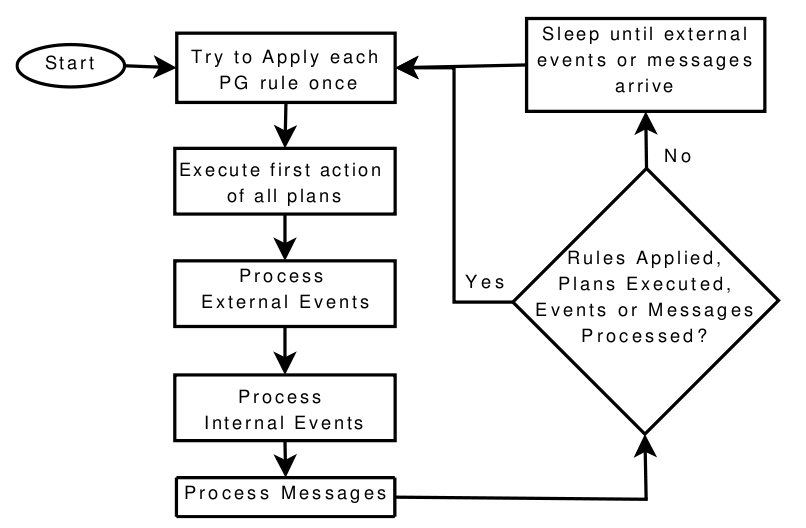
\includegraphics[keepaspectratio,scale=0.3]{fig/rcycle.png}
	\end{center}

	\break

	Properties:
	\begin{enumerate}
		\item If the execution of a plan fails, then the plan will either be repaired in the same deliberation cycle or get re-executed in the next deliberation cycle
		\item If the first action fails and there is no plan repair rule for it, then the failed plan may be successfully executed in the next deliberation cycle
	\end{enumerate}
	
}

%%%%%%%%%%%%%%%%%%%%%%%%%%%%%%%%%%%%%%%%%%%%%%%%%%%%%%%%%%%%%%%%%%%%%%%%
\section{Agent Platform and Tools}
%%%%%%%%%%%%%%%%%%%%%%%%%%%%%%%%%%%%%%%%%%%%%%%%%%%%%%%%%%%%%%%%%%%%%%%%

\frame{
  \frametitle{Agent Platform}
  \begin{itemize}
    \item The 2APL platform is built on the top of JADE (Java Agent DEvelopment Framework).
    \item The fact that 2APL is develop over JADE allows to use all the functionalities that this framework has to communicate to other agents.
    \item As JADE, 2APL follows FIPA specifications.
  \end{itemize}
}

\frame[allowframebreaks]{
  \frametitle{Management of Messages}

  The message agent can be used for sending messages to running agents. The message
  agent can be accessed by clicking on the message agent button in the toolbar.

  \vskip 1.0ex

  We can specify the following elements, as we saw before:
  \begin{itemize}
    \item Receiver, it can be in JADE format.
    \item Performative.
    \item Language (optional)
    \item Ontology (optional)
    \item Content
  \end{itemize}

  \break

  \begin{center}
  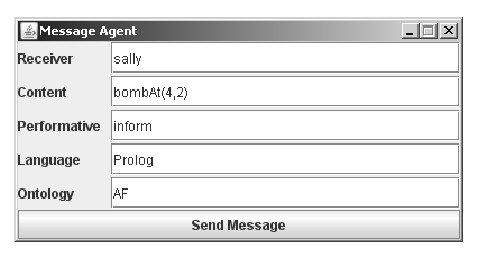
\includegraphics[keepaspectratio,scale=0.75]{fig/messageagent.png}
  \end{center}
}


\frame{
    \frametitle{JADE tools}
\begin{itemize}
    \item 
The RMA (Remote Monitoring Agent) tool - can be used to control the life cycle of the agent platform and of all the registered agents.
    \item 
The sniffer - can be used for tracking messages exchanged in a JADE based environment.
    \item 
The introspector allows to monitor and control the life-cycle of a running agent and its exchanged messages, both the queue of sent and received messages. It allows also to monitor the queue of behaviors, including executing them step-by-step.
\end{itemize}    
}
%%%%%%%%%%%%%%%%%%%%%%%%%%%%%%%%%%%%%%%%%%%%%%%%%%%
\frame{
    \frametitle{RMA: Screenshot}
      \begin{center}
  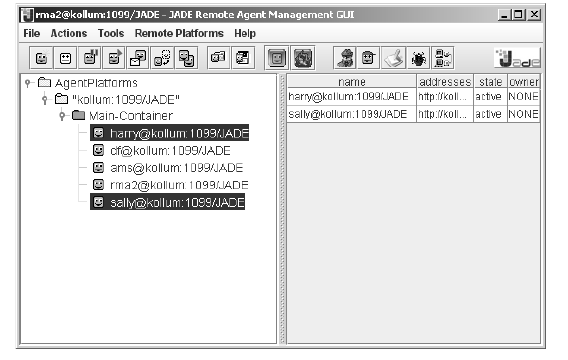
\includegraphics[keepaspectratio,scale=0.5]{fig/rma.png}
  \end{center}
}
%%%%%%%%%%%%%%%%%%%%%%%%%%%%%%%%%%%%%%%%%%%%%%%%%%%
\frame{
    \frametitle{Sniffer: Screenshot}
      \begin{center}
  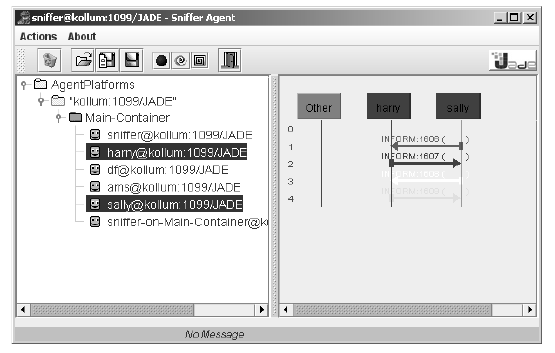
\includegraphics[keepaspectratio,scale=0.5]{fig/sniffer.png}
  \end{center}
}
%%%%%%%%%%%%%%%%%%%%%%%%%%%%%%%%%%%%%%%%%%%%%%%%%%%
\frame{
    \frametitle{Introspector: Screenshot}
      \begin{center}
  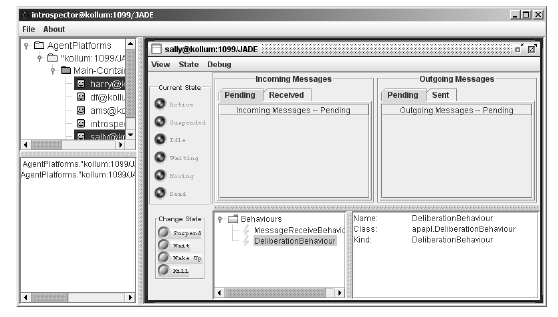
\includegraphics[keepaspectratio,scale=0.5]{fig/introspector.png}
  \end{center}
}
%%%%%%%%%%%%%%%%%%%%%%%%%%%%%%%%%%%%%%%%%%%%%%%%%%%
\frame{
    \frametitle{2APL Specific tools }
\begin{itemize}
    \item The Flexible Graphical Deliberation Cycle (FGDC) tool :
used to visualize and program the deliberation cycle of an agent. The agent’s deliberation cycle is used to determine what the agent should do next.
    \item  The state tracer :
used for showing the execution trace of an agent. Each state shows the beliefs, plans, goals, and log of the agent as a result of executing one deliberation step.

\end{itemize}    
}
%%%%%%%%%%%%%%%%%%%%%%%%%%%%%%%%%%%%%%%%%%%%%%%%%%%
\frame{
    \frametitle{FGDC: Screenshot}
      \begin{center}
  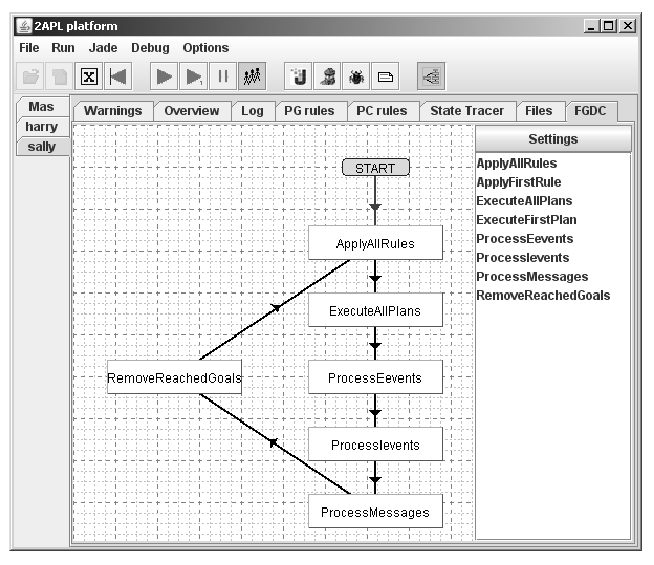
\includegraphics[keepaspectratio,scale=0.5]{fig/fgdc.png}
  \end{center}
}
%%%%%%%%%%%%%%%%%%%%%%%%%%%%%%%%%%%%%%%%%%%%%%%%%%%
\frame{
    \frametitle{State Tracer: Screenshot}
  
    \begin{center}
      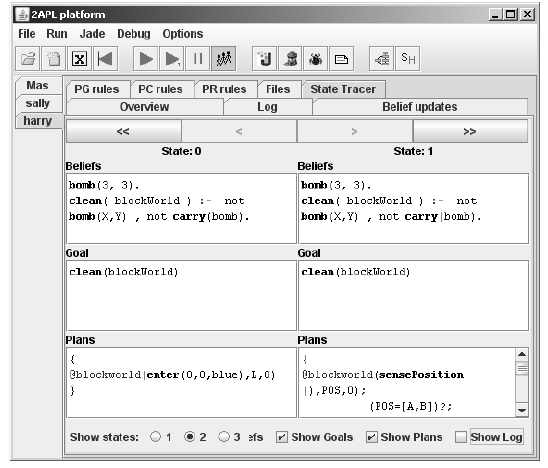
\includegraphics[keepaspectratio,scale=0.5]{fig/state.png}
    \end{center}
  
}
%%%%%%%%%%%%%%%%%%%%%%%%%%%%%%%%%%%%%%%%%%%%%%%%%%%
\frame{
    \frametitle{Environments}

\begin{itemize}
    \item 2APL agents can interact with environments that are implemented in Java.
    \item  You can implement your own environment, or use the “blockworld” environment that is provided by the 2APL platform.
    \item  An environment is specied by a Java class of which one instance
is created by the 2APL platform when loading a multi-agent specication.
    \item  2APL can be ported to other environments , e.g : Bos Wars
\end{itemize}    

}
%%%%%%%%%%%%%%%%%%%%%%%%%%%%%%%%%%%%%%%%%%%%%%%%%%%%%%%%%%%%%%%%%%%%%%%%%
%\section{Demo}			%% BORJA
%%%%%%%%%%%%%%%%%%%%%%%%%%%%%%%%%%%%%%%%%%%%%%%%%%%%%%%%%%%%%%%%%%%%%%%%%

%\frame{
 %\frametitle{Demo}
%}

\frame{
    \frametitle{Block World Environment}

\begin{itemize}
    \item The blockworld is an external environment in which agents can perform actions. 
    \item  The blockworldconsists of a n x n world where agents can move in four directions (north, south, east and west).
    \item  The world can contain bombs, stones, and traps. Agents can pickup and drop bombs.
\end{itemize}    

}
%%%%%%%%%%%%%%%%%%%%%%%%%%%%%%%%%%%%%%%%%%%%%%%%%%%
\frame{
    \frametitle{Block World Environment : Screenshot}
      \begin{center}
  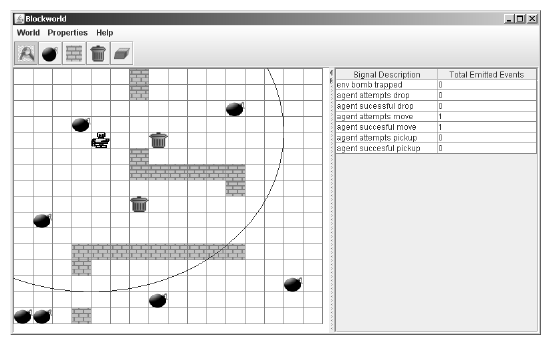
\includegraphics[keepaspectratio,scale=0.5]{fig/block.png}
  \end{center}
}
%%%%%%%%%%%%%%%%%%%%%%%%%%%%%%%%%%%%%%%%%%%%%%%%%%%
\frame{
    \frametitle{Bos Wars Environment}

\begin{itemize}
    \item Bos Wars  is an open source, cross-platform real-time strategy game. The project was started by Tina Petersen in 2004, and the current project leader is François Beerten. The game is written in C++ and Lua with the SDL library.actions. 
    \item  Can be used as an environment for agent testing
    \item  2APL examples available online. There is a great video of a 2APL agent using reinforcement learning to find the optimal strategy for victory.
    \item  http://www.youtube.com/watch?v=mt3Mk5Ea484
\end{itemize}    

}
%%%%%%%%%%%%%%%%%%%%%%%%%%%%%%%%%%%%%%%%%%%%%%%%%%%


%%%%%%%%%%%%%%%%%%%%%%%%%%%%%%%%%%%%%%%%%%%%%%%%%%%%%%%%%%%%%%%%%%%%%%%%
\section{Conclusion}	%% BORJA
%%%%%%%%%%%%%%%%%%%%%%%%%%%%%%%%%%%%%%%%%%%%%%%%%%%%%%%%%%%%%%%%%%%%%%%%

%\frame{
	%\frametitle{Comparison with other languages}
	%SEE LAST PARAGRAPH OF 2APL FULLTEXT PDF 
%}

%%%%%%%%%%%%%%%%%%%%%%%%%%%%%%%%%%%%%%%%%%%%%%%%%%%

\frame{
    \frametitle{Conclusion}
\begin{itemize}
    \item We have presented a brief description of the 2APL language. It is still a rather new language and thus is still fully in development: declarative goals, goal revision rules, nested beliefs, model checking, formal semantics, implementations, etc.

    \item  Active community will help improve it. Already being used in several projects and thesis.
\end{itemize}    
}
%%%%%%%%%%%%%%%%%%%%%%%%%%%%%%%%%%%%%%%%%%%%%%%%%%%
\frame{
    \frametitle{Future Work}
\begin{itemize}
    \item Work being done on various extensions of both 2APL programming language as well as the development tools in the 2APL platform.

    \item  More programming constructs on
    \begin{itemize}
        \item  multi-agent level : to allow the implementation of social and
organisational issues such as norms, obligations, prohibition, permissions, power relation,
delegations of tasks, responsibility, and trust
    
        \item  individual agent level : to allow the implementation of various goals types such as perform, achieve, and maintenance goals.

    \end{itemize}    
    \item  Extending the 2APL platform with (visual) debugging tools that allow
an agent programmer to monitor the execution of multi-agent programs, halt their executions
by means of break points, inspect the mental states of individual agents, and analyze the
interactions among individual agents.
\end{itemize}    
}


%\frame{
% \frametitle{Conclusion}
%}

\begin{frame}{Bibliography}
\nocite{*}
\bibliographystyle{plain}
\bibliography{2apl-pres}
\end{frame}

\end{document}
